\section{Experiments}

It is now time to investigate, how the two efficient algorithms that
we derived in the previous section behave on real world datasets,
both in the context of maximum likelihood estimation as well as
in a Bayesian setting.
In order to do so, we selected three benchmark datasets in advance
that will be used to compare both algorithms to each other as
well as to the baseline uniform sampling procedure, where each
sample is simply selected with equal probability.

It is important to emphasize, that the datasets used in the evaluation
are not a result of cherry picking: We selected the same datasets
as \cite{on-coresets} as well as \cite{coresets-strengthened}
in order to be comparable to other works in the field, without
testing in advance if our algorithms look good on them or not.

Finally, we note that all of the following experiments were
implemented in Python and executed on an
AMD Ryzen 7 2700x processor with 8 cores of 3.7GHz clock speed
and 16GB of RAM.
The code for all the experiments is open source and can be
found publicly accessible on Github.\footnote{
    \url{https://github.com/cxan96/efficient-probit-regression}
}

\subsection{Datasets}

The datasets that are used in the empirical evaluation of our
algorithms are called Covertype\footnote{
    \url{https://archive.ics.uci.edu/ml/datasets/Covertype}
}, Kddcup\footnote{
    \url{https://kdd.ics.uci.edu/databases/kddcup99/kddcup99.html}
} and Webspam\footnote{
    \url{https://www.csie.ntu.edu.tw/\~cjlin/libsvmtools/datasets/binary.html\#webspam}
} and are
all publicly available.

The Covertype dataset consists of $n=581012$ observations of 30x30m
forest patches of wilderness areas located in the
Roosevelt National Forest of Northern Colorado, USA.
The task is to predict the so called covertype of each of these
patches, i.e. the dominant tree species, based on $d=54$
observed features. There are seven distinct tree species that
appear in the dataset, so we have a multiclass problem. To transform
the problem into a binary classification problem that can be
subjected to a probit analysis, we adapted the task to distinguish the
tree species "Lodgepole Pine" from the other six species, thus
obtaining a balanced problem of $49\%$ positive vs. $51\%$ negative
observations.
As an additional preprocessing step, all continuous features of the
dataset were scaled to have a mean of zero as well as unit variance.
In addition, an intercept column of all ones was appended to the data.

The Webspam datasets consists of $n=350000$ observations of
web pages, that can either be classified as spam or no spam, based
on the occurence of 254 distinct words on the web page.
$61\%$ of the observations in the dataset are labeled as spam
and the other $39\%$ are labeled as no spam. The task is to predict,
whether a given web page is spam or not.
The features consist of binary $0/1$ observations that indicate, if
a given word is present on a web page or not.
In a preprocessing step, words that are never present
in the dataset were removed, as well
as words that are only present on a single web page.
After preprocessing, the dataset that is subjected to the
experiments consists of $d=128$ binary features.
An intercept column of all ones was appended to the Webspam dataset
as well.

The Kddcup dataset consists of $n=494021$ observations of network
connections, where the task is to predict if a connection is
"good" or "bad", i.e. to distinguish, whether a hacker tried
to gain unauthorized
access to a network or whether someone tried to establish a
normal and authorized connection.
$80\%$ of the connections in the dataset are "bad" and the other
$20\%$ are "good" connections.
In a preprocessing step, $d=33$ continuous features
were retained from the data and scaled to a mean of zero and
unit variance. Just like the other datasets, an intercept column
of all ones was appended to the Kddcup data as well.

\subsubsection{A Visual Comparison of the Datasets}

Before we evaluate the three competing algorithms on each of
the datasets, we first make an attempt at uncovering some of
the structural characteristics of the data, that could
potentially help us to learn more about the situations in which
the algorithms perform well or might fail.

In order to do so, we first project each dataset onto
its first two principal components, which were obtained
as a result of a principal component analysis
\cite{principal-components}.
The first two principal components are orthogonal vectors that
represent the two directions of the data,
in which the highest variance occurs.
By projecting each datapoint onto the subspace spanned by
the first two principal components, we have
a way of visualizing the datasets in a two dimensional space, while
still retaining as much variance as possible, even though we are
reducing the dimensionality to only 2.

Next, we draw two distinct samples from the reduced datapoints,
each consisting of 500 points. The first one is a uniform sample,
where each datapoint is sampled with equal probability.
The second sample is drawn with probabilities that are proportional
to the statistical leverage scores of the observations with
respect to the original dataset, without applying a PCA.
Both of these samples are presented for each of the datasets in
Figure~\ref{fig:dataset-comparison}.

\begin{figure}[t!]
    \centering
    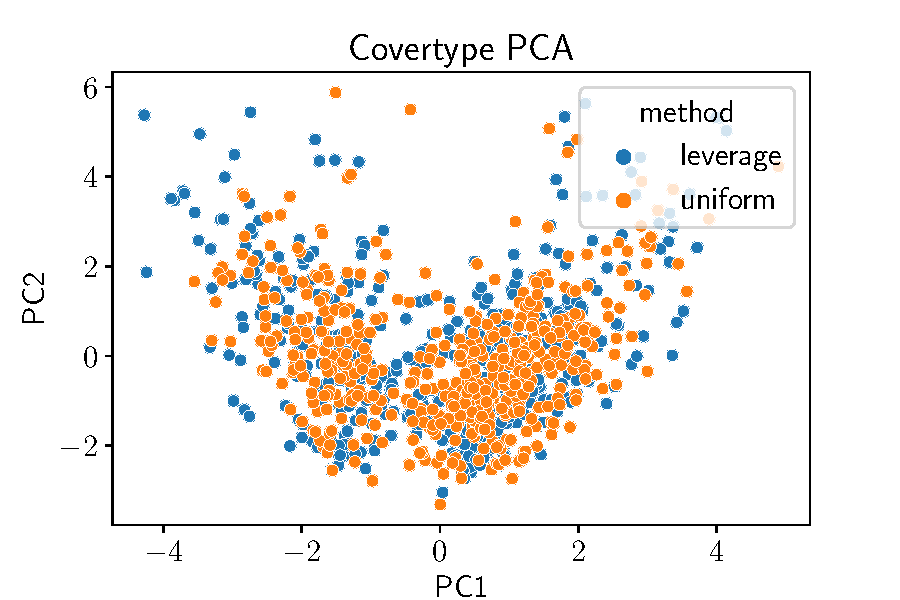
\includegraphics[width=.49\linewidth]{figures/covertype_pca.pdf}
    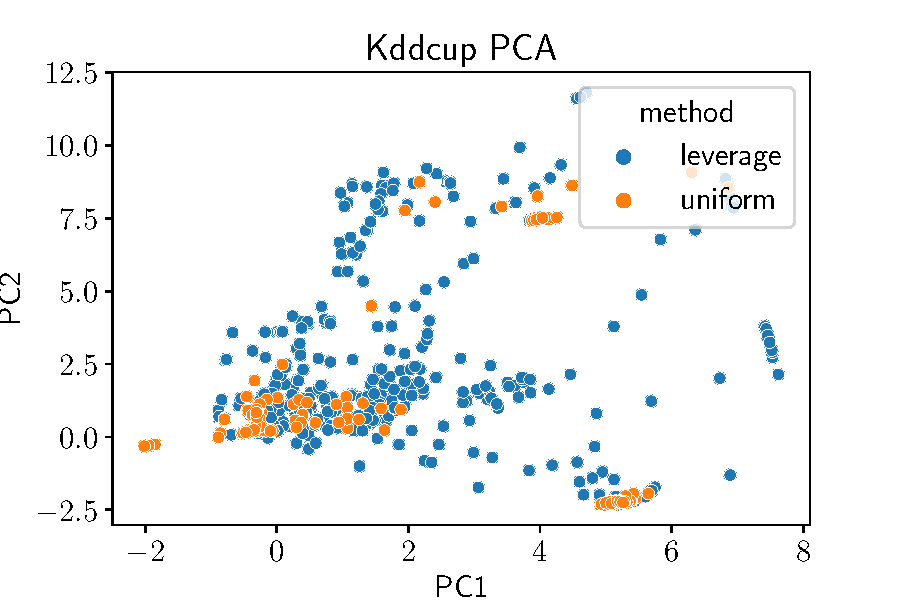
\includegraphics[width=.49\linewidth]{figures/kddcup_pca.pdf}
    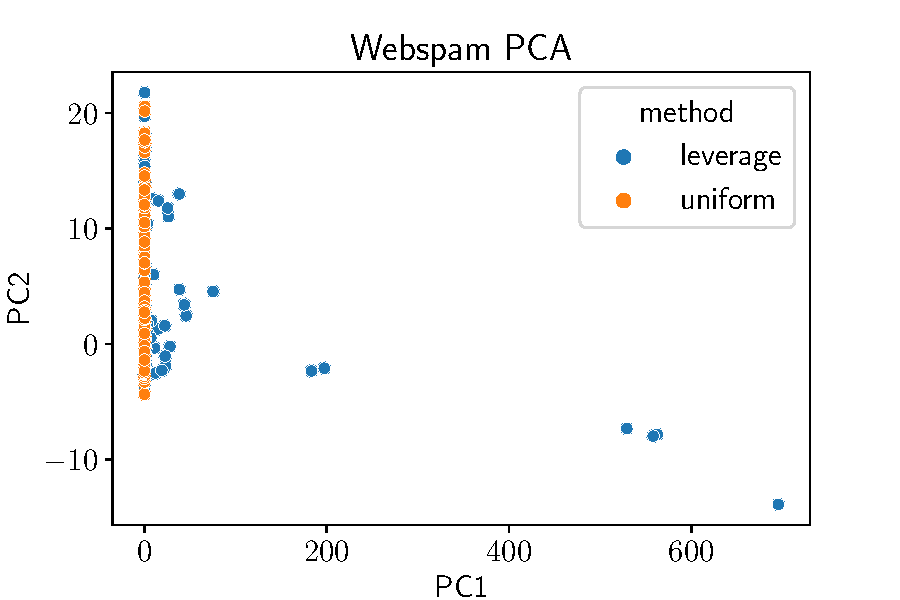
\includegraphics[width=.49\linewidth]{figures/webspam_pca.pdf}
    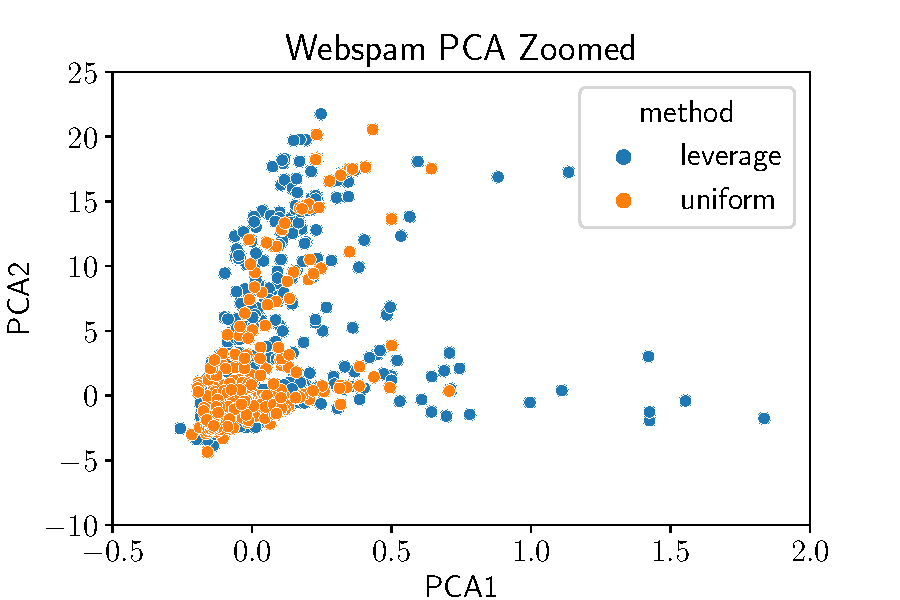
\includegraphics[width=.49\linewidth]{figures/webspam_pca_zoomed.pdf}
    \caption{The datasets are compared by projecting the datapoints
        onto the first two principal components and then drawing
        a random sample of 500 points (a) uniformly and (b) proportionally to the
        statistical leverage scores of the original data.}
    \label{fig:dataset-comparison}
\end{figure}

We can see, that the samples reveal some interesting characteristics
of the datasets. Starting with Covertype, we notice that there
hardly seems to be any difference between the uniform sample and
the leverage score sample. Taking into consideration, that the
statistical leverage scores assign a higher importance to
outliers or "unusual" datapoints, we can conclude that there don't
seem to be too many unusual observations within the Covertype
dataset, or else the two samples would differ more substantially.
It seems to be the case, that a uniform sample is already
sufficient to capture most of the inherent structure of the data,
without having to put extra weight on unusual datapoints, which
simply appear not to exist in this dataset.
Thus, from now on, it seems reasonable to think of the
Covertype dataset as being
a representative for such situations, where the data is
already quite uniformly distributed and not a lot of outliers are
present, i.e. where a uniform sample already seems to
represent the data well.

In contrast to Covertype, the Kddcup dataset exhibits a different
picture. Here, we can see that the uniform sample and the leverage
score sample differ way more substantially than it was the case
for the Covertype dataset.
While the uniform sample only seems to occupy a very limited portion
of the feature space, most of it being a cluster of
many points close to the origin,
the leverage score sample covers a lot more
of the feature space,
indicating that there are a variety of unusual datapoints,
or outliers present,
which the uniform sample misses.
Thus, it seems that we can think of the Kddcup dataset as an
example of a situation,
where on the one hand, we have a lot of similar observations that
are concentrated within a comparatively small proportion of
the feature space, but on the other hand, we also have a
considerable amount of unique observations, which are scattered
around the feature space
while seemingly not belonging to any particular cluster.

Lastly, another interesting situation is presented to us when taking
a look at the two samples of the Webspam dataset.
What strikes the eye first, is that there seem to be some truly
extreme outliers present in the dataset, that the leverage score
sampling picked up on. Only by zooming in on the more crowded area
of the feature space and thereby ignoring those extreme outliers,
we can see the remaining parts of the two samples, which seem to
be rather similar, just like in the situation of the Covertype dataset.
It thus seems to be the case, that the Webspam dataset is an example
of a situation, where on the one hand, the vast majority of the
datapoints are concentrated around some region of the feature space,
but on the other hand, there are also a few hard hitting outliers present,
which exhibit enormous differences from the majority of the other
observations.

\subsection{Coreset-Based Maximum Likelihood Estimation}

We are now ready to investigate, how well our three algorithms
(two pass coreset construction, online coreset construction and
uniform sampling) perform at the task of data reduction
with the goal of estimating the
parameter vector of a probit model on the three datasets that
we just introduced via maximum likelihood estimation.
In order to do so, we present the following experimental setup:

For each of the datasets, we first obtain the objective function
$f(\beta)$ of the original optimization problem without applying
any data reduction and then solve the problem to find the
unique solution $\beta^{opt}$.
Next, we apply our data reduction algorithms in order to select
a small subset of the original data, yielding the reduced
objective function $\tilde{f}(\beta)$. We solve this
smaller optimization problem in order to obtain the solution
$\tilde{\beta}$. Our goal is to see, if the solution on the
reduced dataset, $\tilde{\beta}$, is also a good solution
for the original problem. In order to evaluate the approximation
quality, we compute what we call the approximation ratio:
\begin{equation*}
    \operatorname{approximation\ ratio} = \frac{f(\tilde{\beta})}{f(\beta^{opt})},
\end{equation*}
which always evaluates to a real number in the interval $[1, \infty)$.
The closer this value is to $1$, the better is the quality of
the approximation.

We run this procedure for each algorithm on each of the datasets
for multiple different reduction sizes. Because the algorithms
are not deterministic, we ran each of the experiments a total
of 51 times. The resulting medians as well as the normalized
inter quartile range can be seen in Figure~\ref{fig:ratio-plots}.

\begin{figure}[t!]
    \centering
    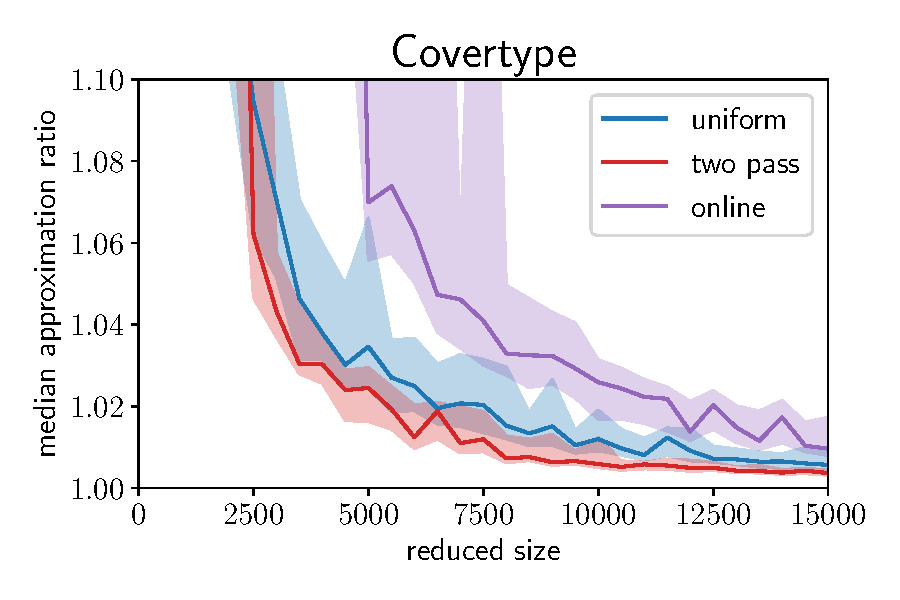
\includegraphics[width=.49\linewidth]{figures/covertype_ratio_plot.pdf}
    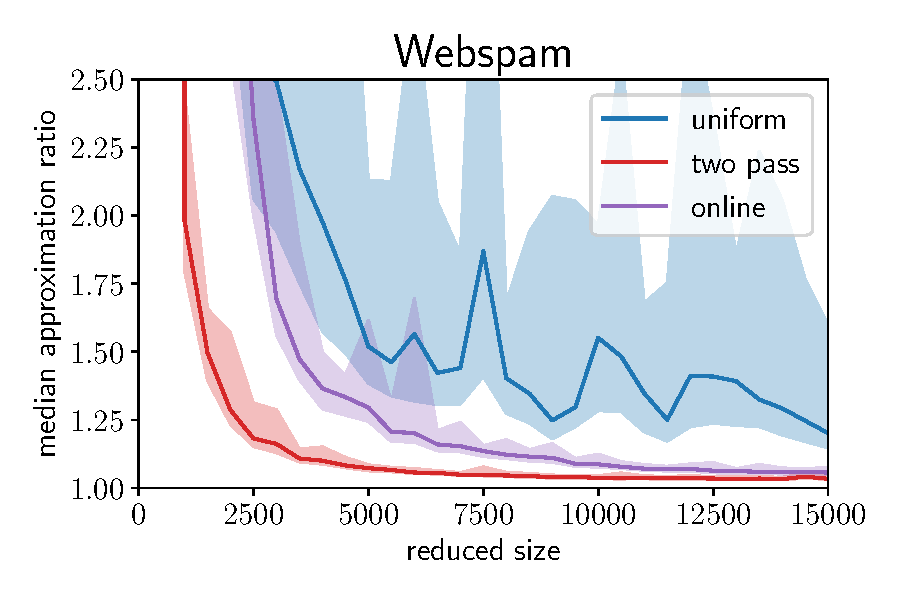
\includegraphics[width=.49\linewidth]{figures/webspam_ratio_plot.pdf}
    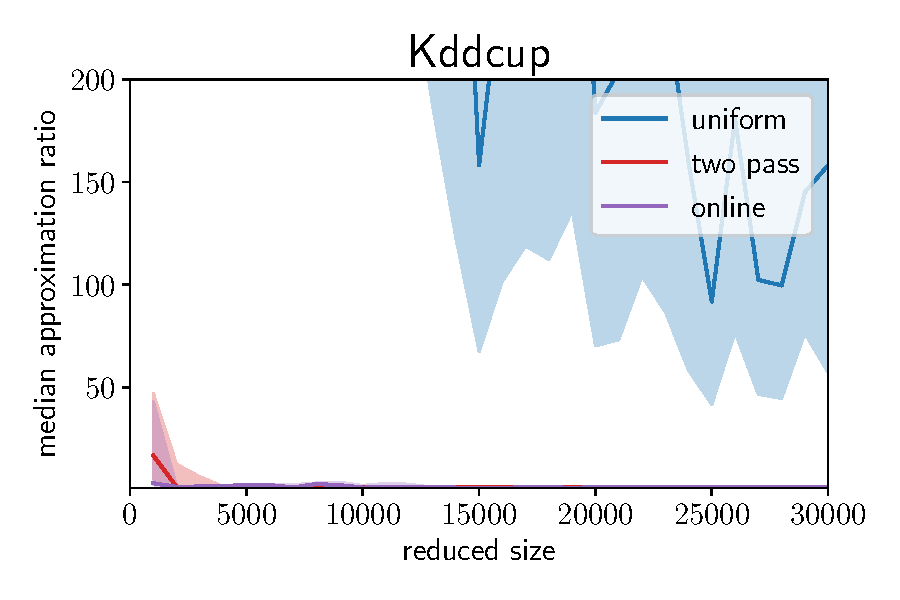
\includegraphics[width=.49\linewidth]{figures/kddcup_ratio_plot.pdf}
    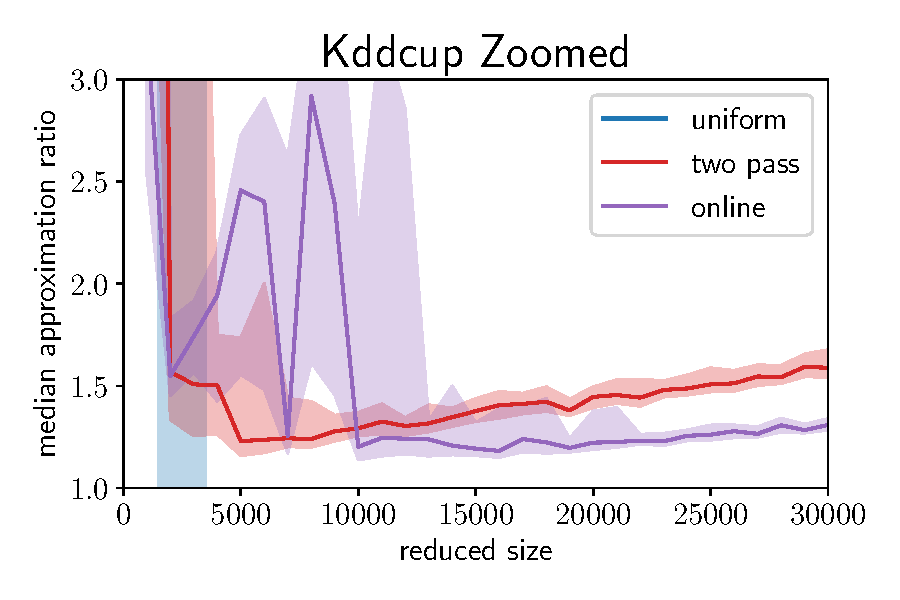
\includegraphics[width=.49\linewidth]{figures/kddcup_ratio_plot_zoomed.pdf}
    \caption{The medians as well as the normalized inter quartile
        ranges of the approximation ratios of the three
        algorithms uniform sampling, two pass coreset construction and
        online coreset construction on the datasets Covertype, Webspam
        and Kddcup for different data reduction sizes.
        For each reduction size, the experiments were repeated a
        total of 51 times.}
    \label{fig:ratio-plots}
\end{figure}

\subsubsection{Comparison of Approximation Quality}

Starting with the Covertype dataset, we can see that each algorithm
quickly reaches good approximation ratios of less than $1.02$
for subset sizes of only $15000$ datapoints, which are less than
$3\%$ of the original dataset.
Both, the uniform sampling as well as the two pass algorithm, are
close to each other in terms of approximation quality, although
the median ratio of the two pass algorithm is always better than
that of uniform sampling. The online algorithm performs worse than
the two competing algorithms, but it also quickly reaches a low
approximation ratio of less than $1.02$.
Interestingly, the fact that the results of our three algorithms
don't differ much on the Covertype dataset, could
be explained by our earlier
findings regarding the characteristics of the data.
For the Covertype dataset, we found that it could be a representative for
those situations, where the datapoints are already
quite homogeneously distributed, i.e. there
are not a lot of outliers, heavy hitters or other unusual points to worry
about and thus, a uniform sample can already be sufficient to
capture the relevant characteristics of the data.
Nevertheless, our two pass algorithm still outperformed the uniform
sampling procedure, albeit by only a small margin.

For the Webspam dataset, the picture looks a lot different. Here,
we can see for the first time, that the uniform sampling algorithm
fails, while the two pass algorithm as well as the one pass
algorithm quickly reach low approximation ratios. On top of that,
the approximation ratios of the uniform sampling algorithm
exhibit a much higher degree of variation and thereby show a lot
less stability than the competing algorithms two pass and online.
Again, it is interesting to note, that these results could also
potentially be explained by our earlier observations:
When visualizing the Webspam dataset by using the first two
principal components, we already noticed that there are a few
extreme outliers present in the data. We also noticed, that
the uniform sample was unable to pick up on those outliers
and only concentrated on the bulk of the datapoints at
the center of the feature space. Now, in our
maximum likelihood experiments,
we can see that the uniform sampling procedure also
exhibits major weaknesses
for the Webspam dataset. It thus seems reasonable to assume,
that this is again happening because the uniform sampling
algorithm misses the extreme outliers, which could potentially have a
high impact on the objective function.
Both, the two pass algorithm as well as the online algorithm,
don't miss those important points thanks to their more
adaptive importance sampling distributions that also take
the statistical leverage scores into account, and therefore show a
stable convergence behavior towards low approximation ratios.

The most dramatic differences between uniform sampling and the
competing algorithms can be observed when looking
at the results for the Kddcup dataset. Here, we can see that
uniform sampling fails terribly and doesn't even reach
approximation ratios lower than $50$. When zooming in, we can
see that our other two algorithms perform much better, although they
also seem to show some difficulties. It is especially interesting
to note, that the online algorithm seems to perform better than the
two pass algorithm, even though its approximations of the
statistical leverage scores are less accurate.
Together with our earlier observations of the structure of the
Kddcup dataset, it seems that Kddcup is a particularly difficult
dataset to compress. Even though the sampling methods that
also rely on the leverage scores clearly outperform the
uniform sampling algorithm, they also show difficulties with
regards to convergence. We should also note here, that the
maximum size of $30000$ points for the Kddcup dataset already
takes up more than $6\%$ of the whole dataset, which is more than
double as much as what was needed for the Covertype dataset to
achieve a much better approximation quality.
Thus, the Kddcup dataset seems to be more challenging for all the
competing algorithms, although the two pass algorithm and the
online algorithm handle the difficult conditions way better than
the uniform sampling algorithm.

\subsubsection{Comparison of Running Times}
\label{sec:running-times-comparison-ml}

We round off our first experiment with a discussion regarding the
runtimes of the algorithms compared to the time it takes to
solve the original problem without prior reduction, as well as
a discussion of the tradeoffs between approximation quality and
running time.

It must be noted, that the online coreset algorithm
had to be excluded from the comparison due to its
incomparably high running time of $O(nd^2)$, which would have
made it impossible to execute a sufficient number of experiments.
However, we remark that the advantage of the online algorithm isn't
necessarily its speed, but that it is able to construct coresets
even when two passes over the data are impossible and every sampling
decision has to be made immediately. Also, it might be possible
to drastically increase the efficiency of the online algorithm,
by running mutiple parallel instances of it on a distributed
cluster and then equally balancing the load of the incoming
data records between
each of the instances, but these possible adaptations are
left open for future work.

The total running times for obtaining the maximum
likelihood estimate of the probit model for each of the
datasets without applying any data reduction are given in
Table~\ref{tab:running-times} to serve as a
baseline for further discussions.

\begin{table*}[ht!]
    \centering
    \begin{tabular}{ l | l| l| l}
        \hline
                           & \textbf{Covertype} & \textbf{Kddcup} & \textbf{Webspam} \\ \hline
        Total running time & $535$ seconds      & $103$ seconds   & $447$ seconds    \\ \hline
    \end{tabular}
    \caption{The total running times that it takes to obtain the maximum
        likelihood estimator for each of the datasets.}
    \label{tab:running-times}
\end{table*}

In Figure~\ref{fig:runtime-plots}, we present the
tradeoffs between approximation ratio and running time
for uniform sampling as well as for the fast two pass algorithm.
The reported times include the data reduction step as
well as the optimization step, in order to be able to
compare the times to the total running times without data reduction.

\begin{figure}[t]
    \centering
    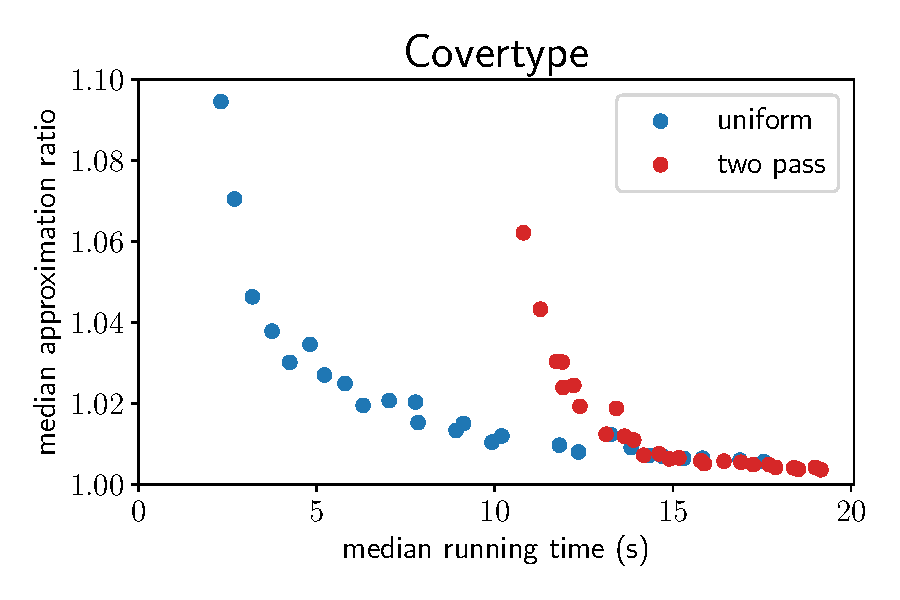
\includegraphics[width=.49\linewidth]{figures/covertype_runtime_plot.pdf}
    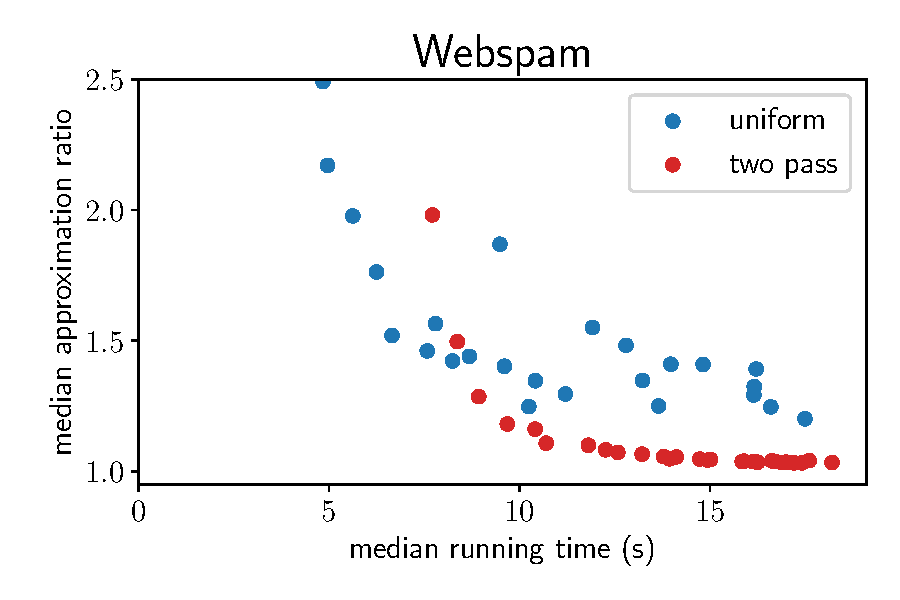
\includegraphics[width=.49\linewidth]{figures/webspam_runtime_plot.pdf}
    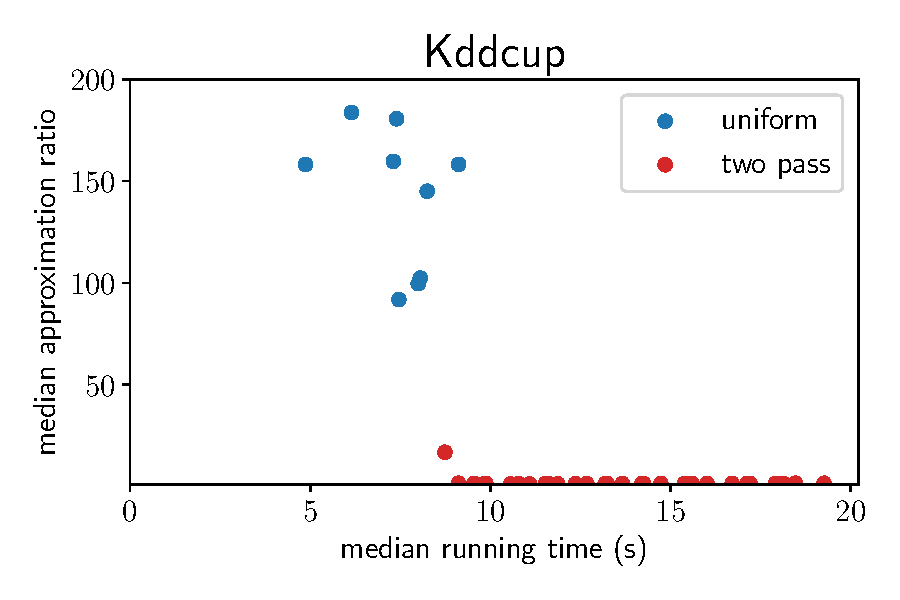
\includegraphics[width=.49\linewidth]{figures/kddcup_runtime_plot.pdf}
    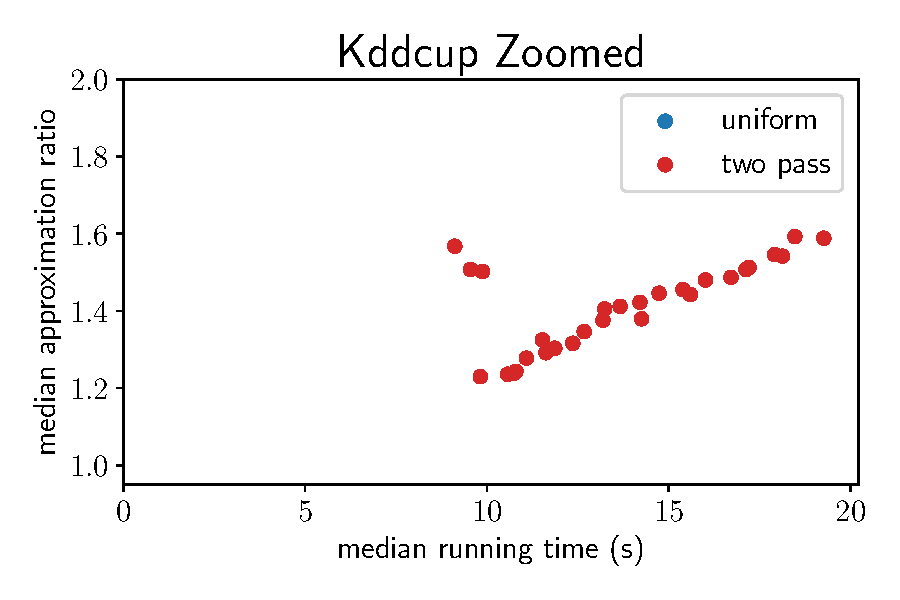
\includegraphics[width=.49\linewidth]{figures/kddcup_runtime_plot_zoomed.pdf}
    \caption{The plots show the tradeoffs between running time and
        approximation ratio for the uniform sampling algorithm and the
        fast two pass algorithm on our datasets.
        Every point represents the median in running time, as well
        as the median in approximation ratio, for a given
        data reduction size.
    }
    \label{fig:runtime-plots}
\end{figure}

When looking at the results for the Covertype dataset, we can see
that the uniform sampling algorithm outperforms the two pass
algorithm in terms of speed, but is unable to reach the same degree
of approximation quality as the two pass algorithm. The running times of
the uniform sampling procedure range roughly between 1 and
10 seconds, but decent results are only achieved when investing
at least 5 seconds. On the other hand, the running times of the
two pass algorithm range between 10 and 20 seconds, thus taking
almost twice as long. But compared to the total running time
for the Covertype dataset without reduction, we can see that
even the two pass algorithm reduces the total running time
to obtain the maximum likelihood estimate
by more than $96\%$, from 535 seconds to less than 20 seconds.

Taking a look at the Webspam dataset, we can see an interesting
picture: Not only does the two pass algorithm show better
approximation rates than the uniform sampling algorithm, but
it also shows similar running times. Thus, for the Webspam dataset,
the two pass algorithm almost dominates the uniform sampling
in the two criterias, since it has similar running times but
achieves a better approximation quality.
For running times of 15 seconds, the fast two pass algorithm already
achieves decent results, thus we can say that the
original time for solving the unreduced problem was again reduced
by more than $96\%$, from 447 seconds to only 15 seconds.

In the case of Kddcup, the comparison is almost pointless, because
the uniform sampling fails. We only include these results to show
that the running times of the two pass algorithm consistently
range between 10 and 20 seconds, even when the data is
substantially less well behaved, as we showed for the
Kddcup dataset. Here, the time savings are not quite as impressive
as for the Covertype and the Webspam dataset:
The total running time was "only" reduced by more than $80\%$,
from 103 seconds to less than 20 seconds. Still, we can
consider this a decent win, especially when keeping
in mind that the uniform sampling algorithm failed completely.

To conclude the discussion of our first experiment, we can
say that the slightly increased running time of the two
pass algorithm compared to the uniform sampling algorithm
should be of no concern, because the few seconds in excess
runtime were always well compensated by substantial
gains in approximation quality. For each dataset,
the two pass algorithm is able to reduce the total
optimization time by more than $80\%$, even $96\%$ for
the Covertype and for the Webspam dataset.

\subsection{Coreset-Based Bayesian Inference}

The goal of our second experiment is to investigate, if our
algorithms can successfully be applied as a data reduction
step to cut down the computational cost of performing
a full Bayesian probit analysis on our three datasets.
In order to do so, we use the efficient Gibbs sampler
described earlier in Section~\ref{sec:gibbs} to generate
samples with and without a preceding data reduction step using
our algorithms, and see how they compare to each other.
But before we can get into the full experimental setup,
we must note that in order to use the Gibbs sampler together
with our algorithms, it has to be slightly adapted
to account for the sample weights that are an
essential component of our coreset algorithms,
which is briefly covered in the next section.

\subsubsection{Adapting the Gibbs Sampler for Weighted Coresets}
\label{sec:gibbs-adaptation}

The first part of the Gibbs sampler that has to be slightly adapted
is the expression $B = (M^{-1} + X^TX)^{-1}$, where
$M \in \mathbb{R}^{d \times d}$
is the prior covariance matrix and
$X \in \mathbb{R}^{n \times d}$ is the model matrix.
When using our algorithms to draw a random sample of $k$
datapoints according to the distribution $p_1, ..., p_n$
and arranging them in a matrix $C \in \mathbb{R}^{k \times d}$,
the matrix $C$ is now random too, because it is the result of
drawing the random sample of our datapoints.
Our goal is now, to find weights $u_1, ..., u_n$ for our
data points, such that when $C$ is a random sample of the
reweighted datapoints $u_1x_1, ..., u_nx_n$, we have
\begin{equation*}
    E[C^TC] \overset{!}{=} X^TX,
\end{equation*}
where $X$ is the model matrix of our original unweighted datapoints.
We can accomplish this by calculating the expected value as follows:
\begin{align*}
    E[C^TC] & = E\left[\sum_{j=1}^k c_jc_j^T\right]
    = \sum_{j=1}^k \sum_{i=1}^n u_i^2 p_i x_i x_i^T \\
            & = k\sum_{i=1}^n u_i^2 p_i x_i x_i^T
    \overset{!}{=} \sum_{i=1}^n x_i x_i^T = X^TX.
\end{align*}
By comparing the coefficients, we see that
$u_i = \frac{1}{\sqrt{k p_i}}$ is the required weight.
Thus, when the Gibbs sampler is applied to a subset
$\mathcal{C}$ of our initial dataset, we need to multiply every
datapoint of the subset with the weight
$u_i = \frac{1}{\sqrt{k p_i}}$, before we can plug it into
the expression for obtaining $B$.

Next, we need to adapt the expression
$X^Ty^\ast$, where $y^\ast$ is the current vector of the latent
variables. We do this in a similar fashion, by asking
how we should reweight the original datapoints as well as the
latent variables in order to be unbiased, i.e. we want that
\begin{equation*}
    E\left[ C^T y_C^\ast \right] = X^T y^\ast,
\end{equation*}
where $y_C^\ast$ is the random sample of the latent variables that
is associated with the random sample in $C$.
Luckily, it turns out, that the weights that we obtained earlier
are also correct for adapting this expression:
\begin{align*}
    E\left[ C^T y_C^\ast \right] = E\left[ \sum_{j=1}^k c_j (y_C^\ast)_j \right]
    = \sum_{j=1}^k \sum_{i=1}^n u_i^2 p_i x_i y^\ast_i
    = k \sum_{i=1}^n \left(\frac{1}{\sqrt{kp_i}}\right)^2 p_i x_i y^\ast_i
    = X^T y^\ast.
\end{align*}

It follows, that when using the Gibbs sampler in conjunction
with our algorithms, we have to reweight our sample with weights
$u_i = \frac{1}{\sqrt{k p_i}}$ both when obtaining $X^TX$ as
well as $X^Ty^\ast$.

\subsubsection{Experimental Setup}

We used a similar experimental setup
as in \cite{scalable-bayesian-logreg} and
\cite{bayesian-regression}:
First, we arbitrarily selected a relatively uninformative
prior distribution of
\begin{equation*}
    \beta \sim \mathcal{N}(0, 10 \cdot \mathcal{I}),
\end{equation*}
where $\mathcal{I}$ is the identity matrix.
Next, we used the Gibbs sampler
to generate a sample of the full posterior
distribution without applying any data reduction for each
of the three datasets.
Each of the three full posterior samples has a size of $10000$,
and for each of the datasets, a different
burn in value was selected. For Covertype, a burn in
of 200 was sufficient, 2000 was needed for Kddcup and 3000
for Webspam.

Next, we applied our algorithms to each of the datasets
for a variety of reduction sizes and ran the adapted version of
the Gibbs sampler (see Section~\ref{sec:gibbs-adaptation} above)
on the reduced data, obtaining a posterior sample of size 1000
for each data reduction size. The burn in values for
the reduced samples were set to be
the same as for the original unreduced data.

Our goal is now to compare the posterior samples that were
obtained by running the Gibbs sampler on the reduced data
to the posterior samples that were obtained from the
original data.
In order to do so, we use a total of three different measures.

The first measure of approximation quality that we
apply compares the mean
of the original posterior distribution without data reduction to
the mean of the posterior distribution with a prior data reduction step,
by evaluating the expression
$\lVert \mu_\beta - \widetilde{\mu}_\beta \rVert_2$,
where $\mu_\beta$ is the mean of the original posterior and
$\widetilde{\mu}_\beta$ is the mean of the reduced posterior.

Likewise, our second measure compares the covariance matrices of
the two samples by evaluating the expression
$\lVert \Sigma_\beta - \widetilde{\Sigma}_\beta \rVert_2$,
where $\Sigma_\beta$ is the covariance matrix of the original
posterior sample without data reduction and
$\widetilde{\Sigma}_\beta$ is the covariance matrix of the
posterior sample with data reduction. The norm $\lVert \cdot \rVert_2$
refers to the spectral norm, which is equal to the
largest singular value.

Our third measure is the maximum mean discrepancy (MMD,
see for example \cite{mmd}),
which was also applied in \cite{scalable-bayesian-logreg}.
The MMD was originally intended to be a test statistic for the
problem of testing, if two samples come from the same
distribution or not.
In order to do so, the idea behind the MMD is to transform
both samples into a higher dimensional space and then to
compare the means of the samples in the new space.
The MMD is then the resulting difference of the means in the
higher dimensional space. It follows, that the higher the
MMD, the more different the two samples are.
In order to transform the samples
into the higher space, the authors of
\cite{scalable-bayesian-logreg} used a so called polynomial
kernel function, and to stay comparable to them, we
use a polynomial kernel as well.

\subsubsection{Comparison of Approximation Quality}

Figure~\ref{fig:bayes-plots-norm-cov} shows the results of our
experiment for the measures
$\lVert \mu_\beta - \widetilde{\mu}_\beta \rVert_2$, which
we from now on call mean distance and
$\lVert \Sigma_\beta - \widetilde{\Sigma}_\beta \rVert_2$,
which we from now on call covariance distance.
The results for the MMD can be found in Figure~\ref{fig:bayes-plots-mmd}.

\begin{figure}[ht!]
    \centering
    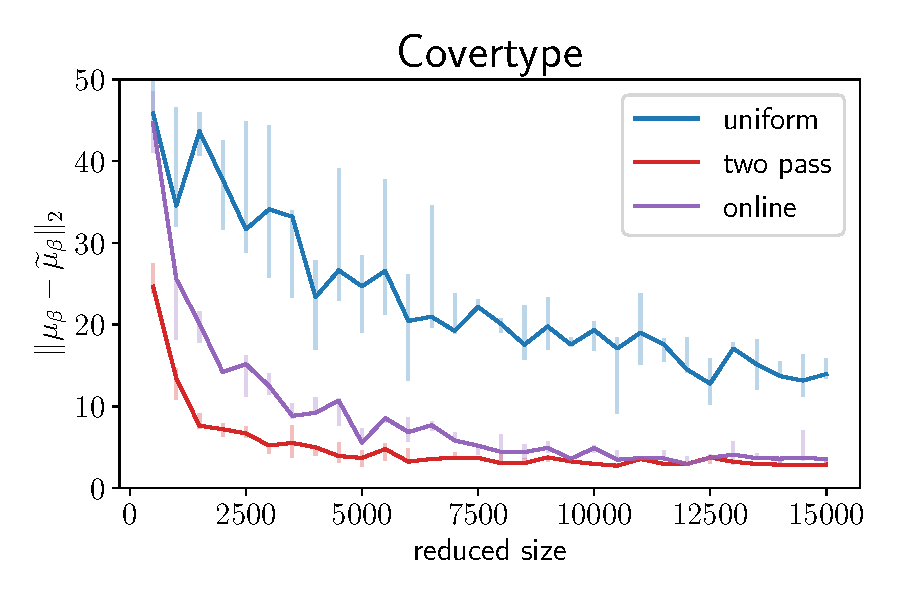
\includegraphics[width=.49\linewidth]{figures/covertype_bayes_plot_norm.pdf}
    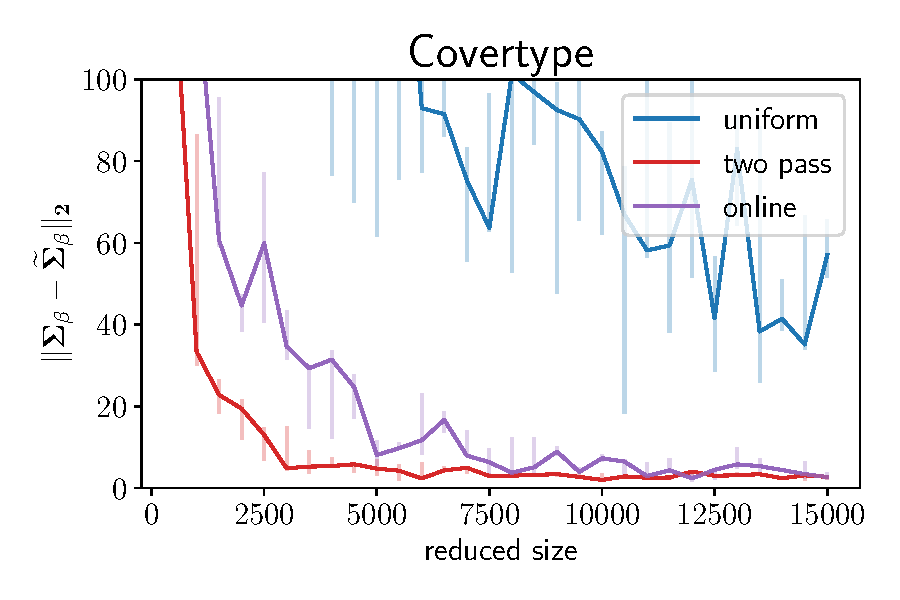
\includegraphics[width=.49\linewidth]{figures/covertype_bayes_plot_matrix_norm.pdf}
    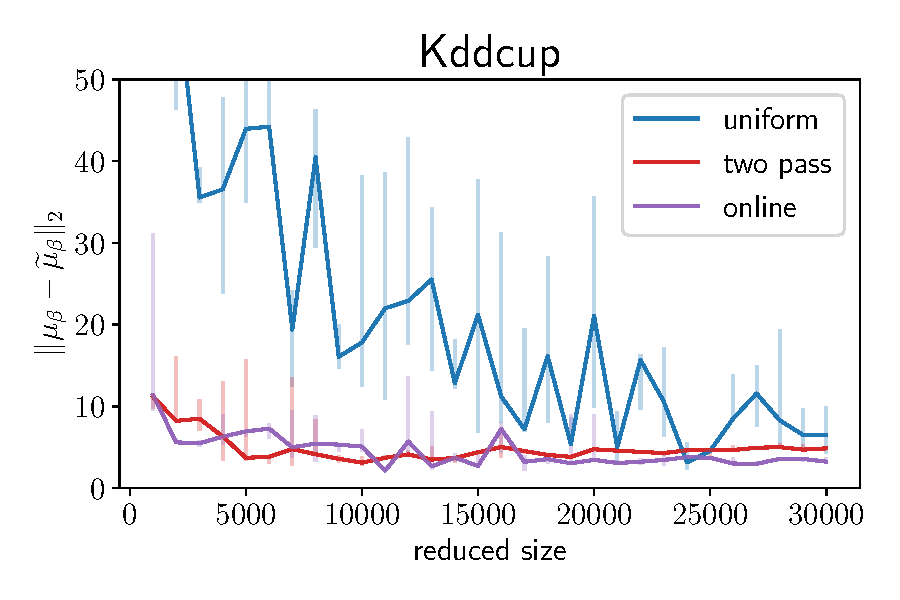
\includegraphics[width=.49\linewidth]{figures/kddcup_bayes_plot_norm.pdf}
    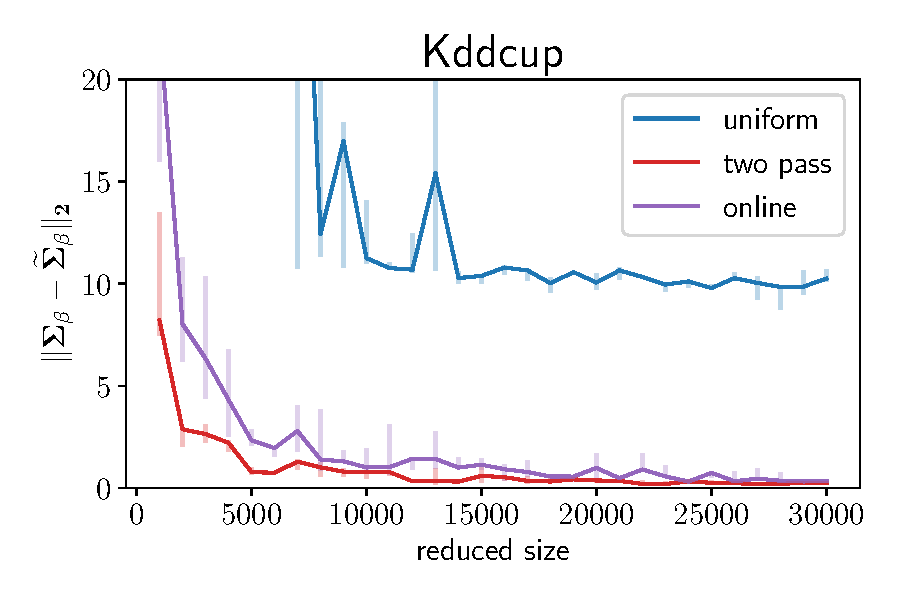
\includegraphics[width=.49\linewidth]{figures/kddcup_bayes_plot_matrix_norm.pdf}
    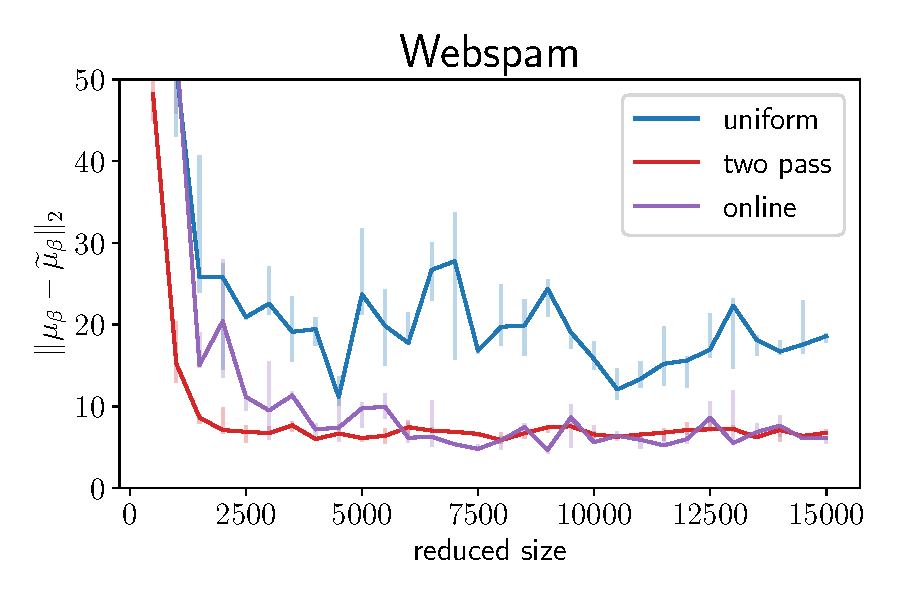
\includegraphics[width=.49\linewidth]{figures/webspam_bayes_plot_norm.pdf}
    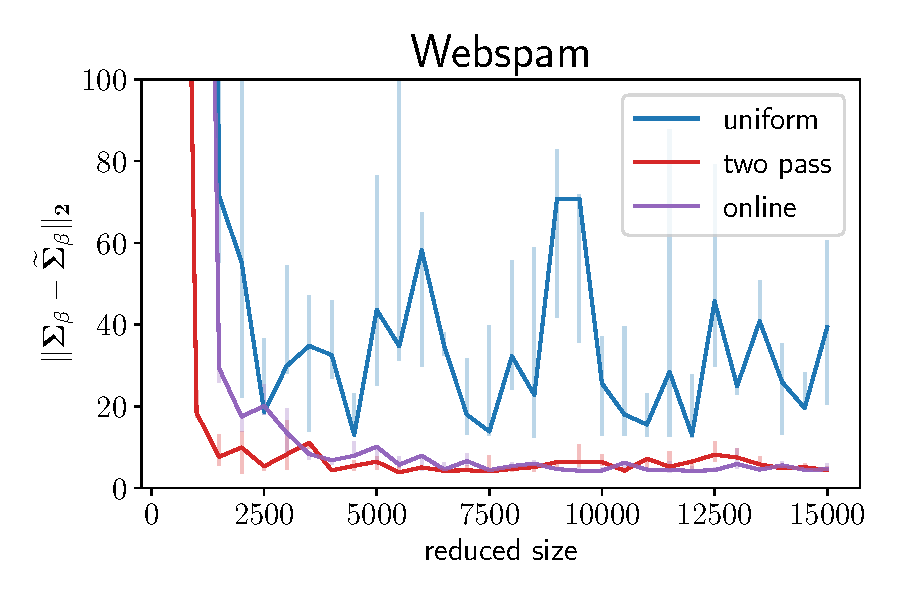
\includegraphics[width=.49\linewidth]{figures/webspam_bayes_plot_matrix_norm.pdf}
    \caption{In the left column, we see the mean distance between the posterior
        distribution sampled after running our algorithms and
        the original posterior distribution sampled without data
        reduction. In the right column, we see the covariance distance for
        our algorithms. Every experiment was repeated a total
        of 5 times, and the solid lines represent the
        medians. The lower and upper error bars indicate the
        $25\%$ quantile as well as the $75\%$ quantile, respectively.}
    \label{fig:bayes-plots-norm-cov}
\end{figure}

\begin{figure}[ht!]
    \centering
    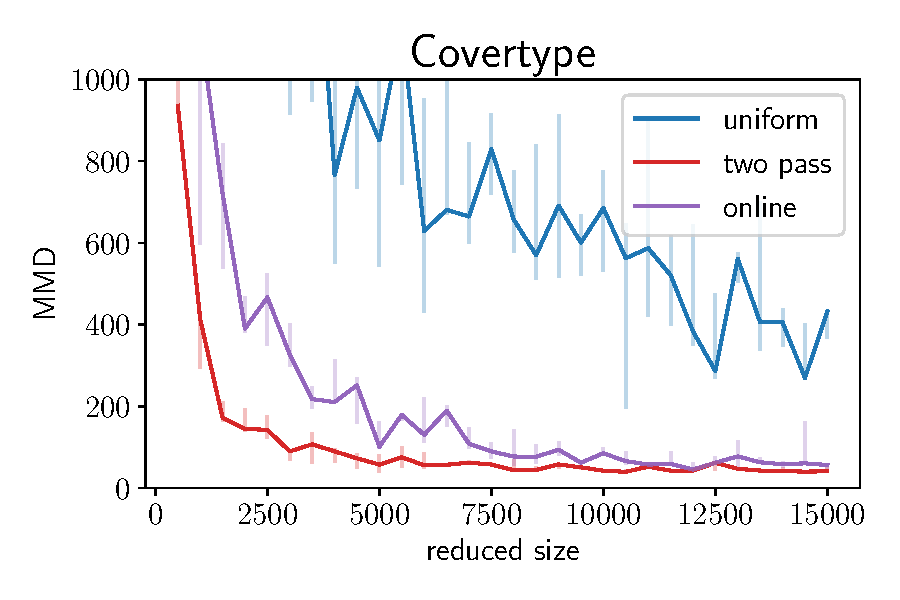
\includegraphics[width=.49\linewidth]{figures/covertype_bayes_plot_mmd.pdf}
    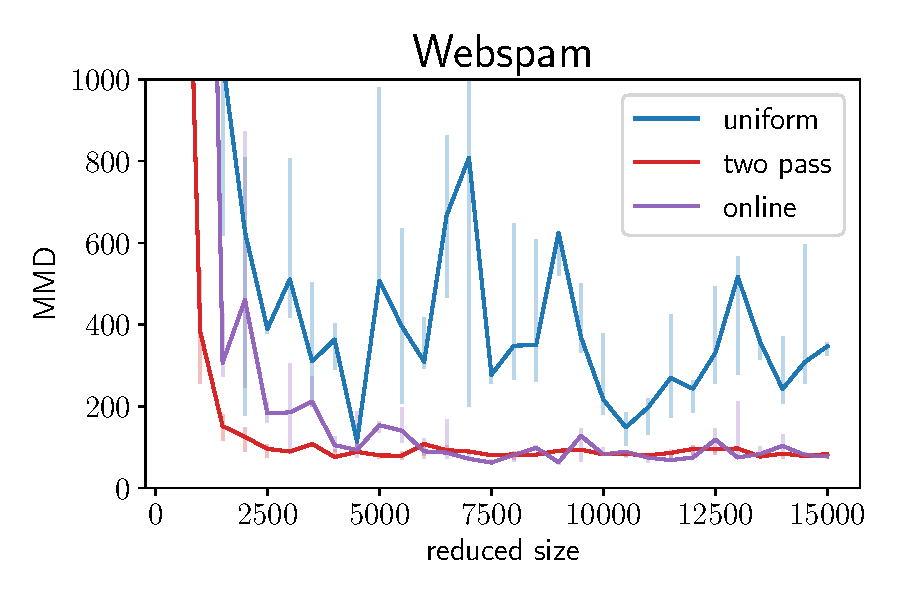
\includegraphics[width=.49\linewidth]{figures/webspam_bayes_plot_mmd.pdf}
    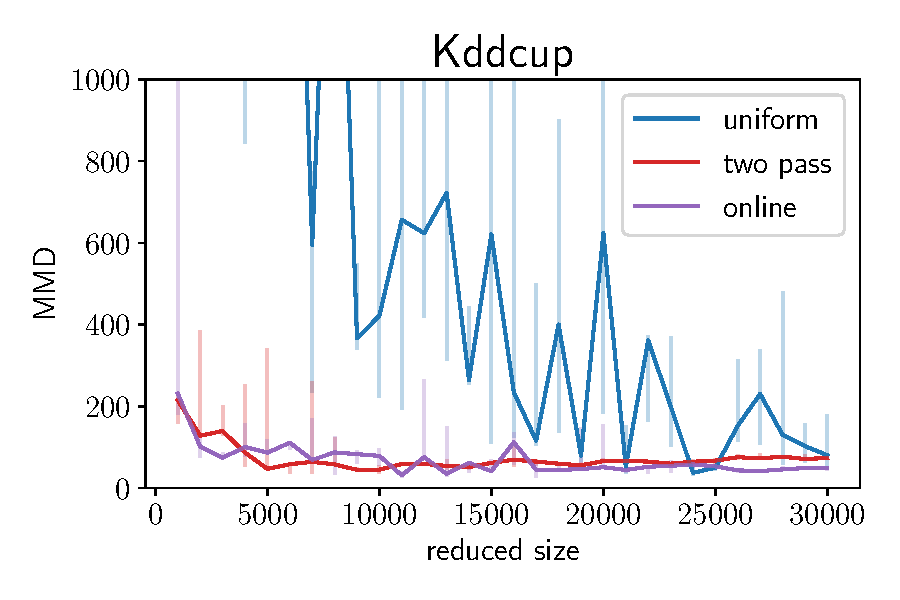
\includegraphics[width=.49\linewidth]{figures/kddcup_bayes_plot_mmd.pdf}
    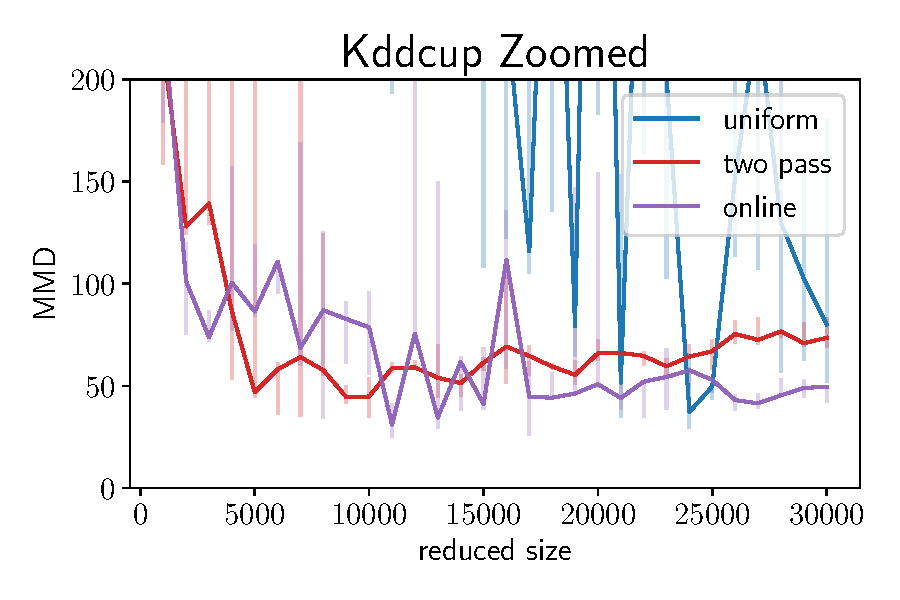
\includegraphics[width=.49\linewidth]{figures/kddcup_bayes_plot_mmd_zoomed.pdf}
    \caption{The MMD for each dataset and multiple data reduction
        sizes. Every experiment was repeated a total
        of 5 times, and the solid lines represent the
        medians. The lower and upper error bars indicate the
        $25\%$ quantile as well as the $75\%$ quantile, respectively.}
    \label{fig:bayes-plots-mmd}
\end{figure}

For the Covertype dataset, we can see that our two algorithms
substantially outperform the uniform sampling algorithm for
each of the three measures. The clearest difference can be
seen when looking at the covariance distance.
While both of our algorithms approach zero even for
reduction sizes of less than 10000, the uniform sampling
has big trouble to even come close to convergence.
This finding suggests, that the samples of the posterior
that were generated after running our algorithms are
substantially closer to the original posterior distribution
in terms of variance, than the samples generated by using the
uniform sampling procedure.
When looking at the other measures for the Covertype dataset,
we can make similar observations: Despite the fact that we
characterized the Covertype dataset to be well behaved for
uniform sampling earlier on, we now observe that the uniform sampling
seems to fail to capture some of the important elements of the
data, which substantially influence the outcome of the Gibbs
sampling procedure.

For the Kddcup dataset, the differences are particularly apparent
when looking at the covariance distance. Here, the uniform sampling
even seems to stagnate, not moving towards zero at all.
Our two algorithms on the other hand don't have the same problem:
Their covariance distance decreases and approaches zero without
any visible trouble.
When looking at the mean distance for the Kddcup dataset, we can
see that our algorithms also outperform, but at least the uniform sampling
comes close for reduction sizes of over 25000.
For the MMD, we can see a similar picture: Our algorithms clearly
outperform, but the uniform sampling at least comes closer
for the higher reduction sizes, although the error bars indicate
a much higher degree of instability.

When looking at the Webspam dataset, we can see a similar picture
like we already saw for the other two datasets. For each
of the three measures, uniform sampling exhibits substantial
problems, while our leverage score based algorithms seem to
deliver much higher quality approximations.

To conclude the discussion on approximation quality, we compare
a concrete sample of the posterior, that was created by using each
of the three algorithms with a reduction size
of 15000, to the original posterior sample of the Covertype dataset.
In Figure~\ref{fig:covertype-coefficients-1} and
Figure~\ref{fig:covertype-coefficients-2}, we present boxplots to
visualize the samples for each of the coefficients.

\begin{figure}[ht!]
    \centering
    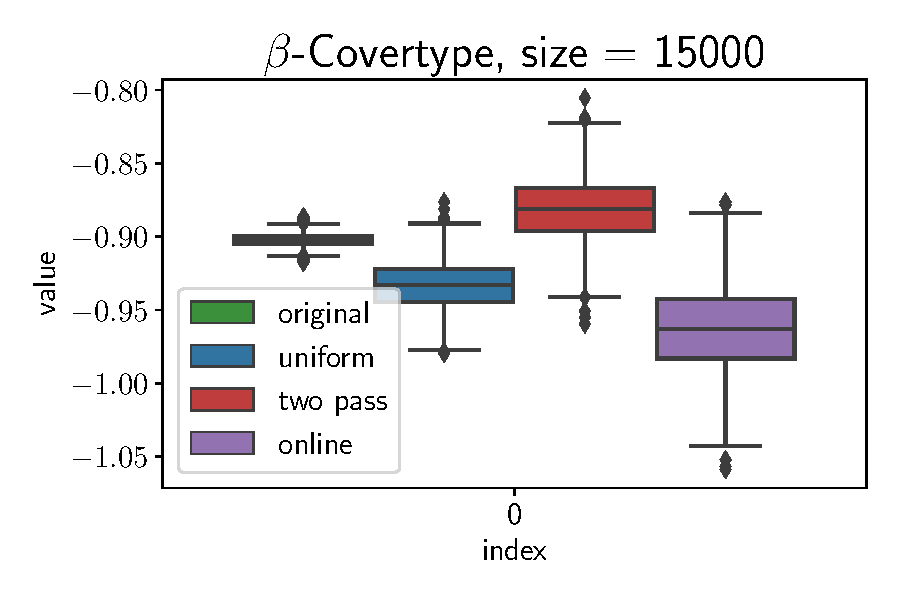
\includegraphics[width=.49\linewidth]{figures/covertype_coefficients/covertype_coefficients_0.pdf}
    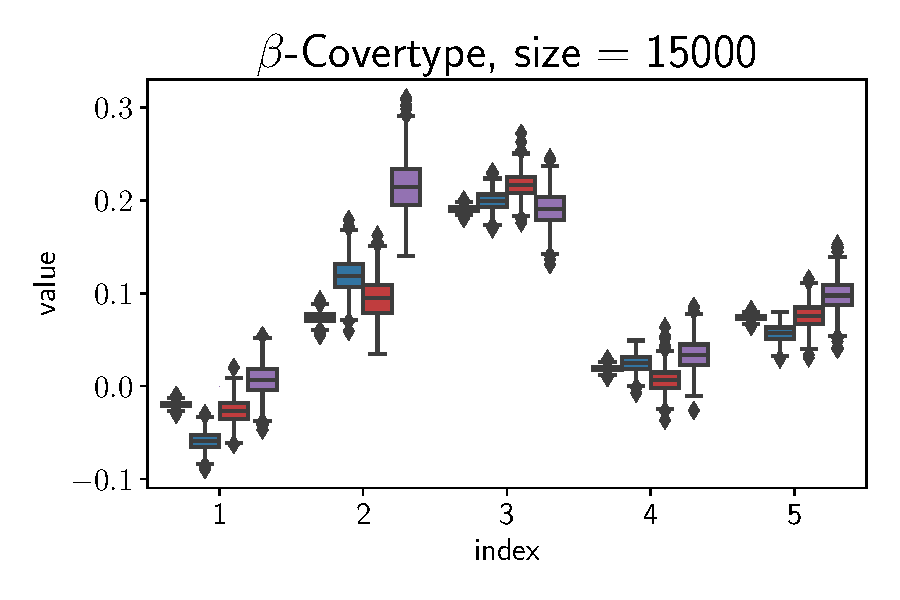
\includegraphics[width=.49\linewidth]{figures/covertype_coefficients/covertype_coefficients_1.pdf}
    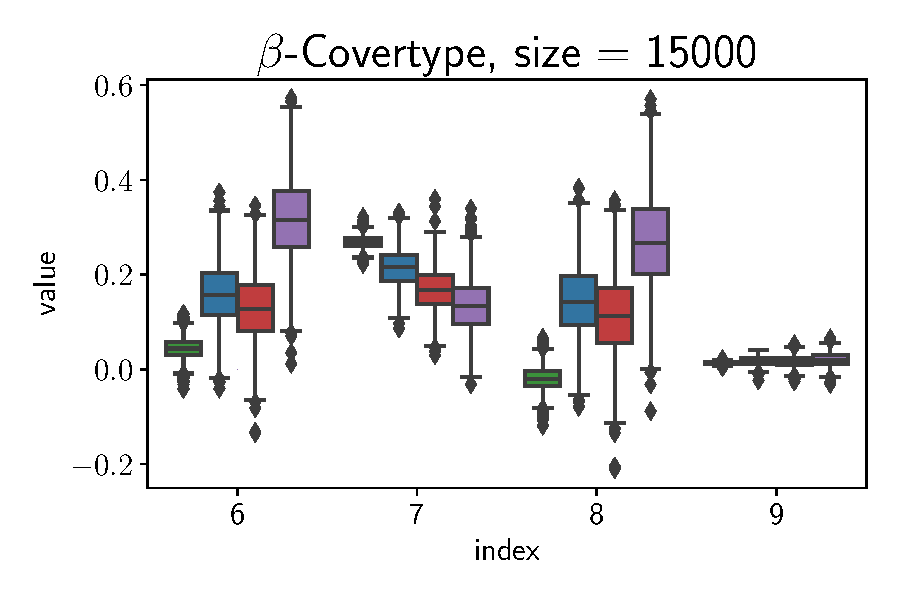
\includegraphics[width=.49\linewidth]{figures/covertype_coefficients/covertype_coefficients_6.pdf}
    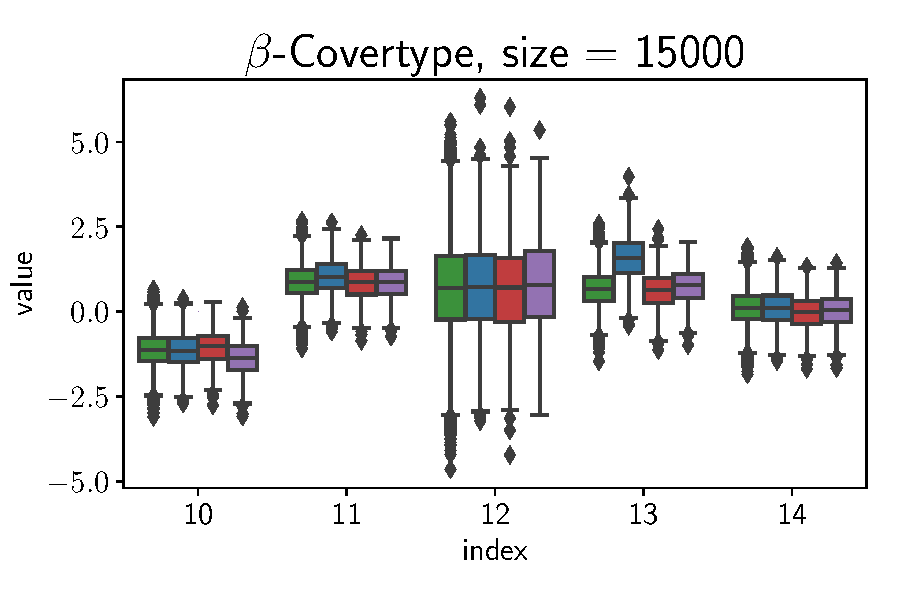
\includegraphics[width=.49\linewidth]{figures/covertype_coefficients/covertype_coefficients_10.pdf}
    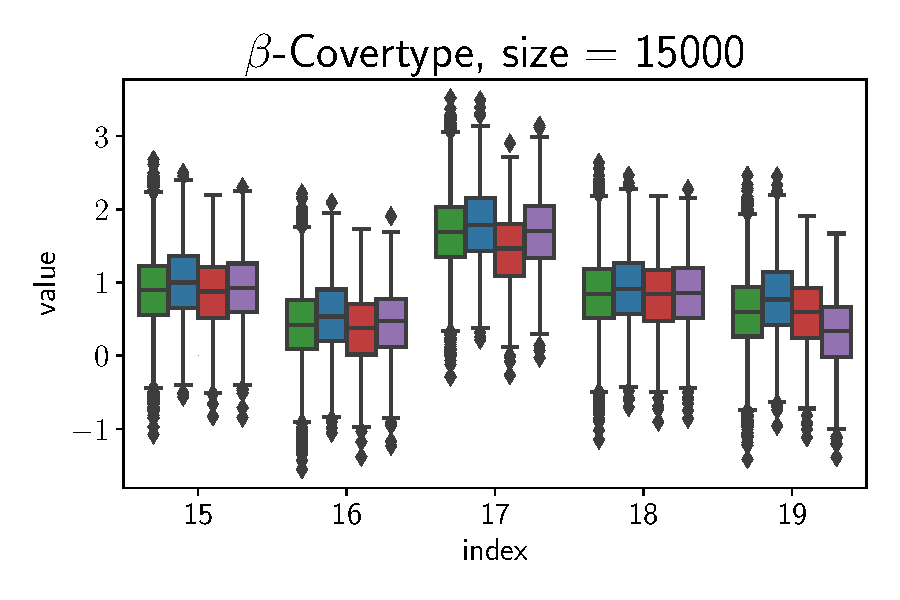
\includegraphics[width=.49\linewidth]{figures/covertype_coefficients/covertype_coefficients_15.pdf}
    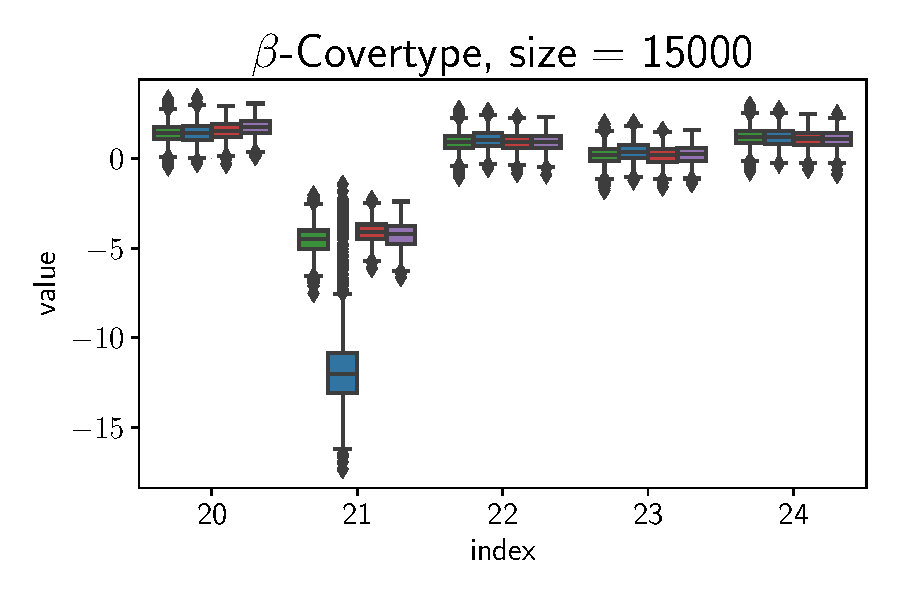
\includegraphics[width=.49\linewidth]{figures/covertype_coefficients/covertype_coefficients_20.pdf}
    \caption{The posterior samples obtained after running each of
        the algorithms for a reduction size of 15000 are compared to
        the original sample of the posterior distribution of the
        Covertype dataset by using
        boxplots for each of the dimensions of $\beta$.
        Here, we can see $\beta_0$ to $\beta_{24}$, the remainder can
        be found in Figure~\ref{fig:covertype-coefficients-2}.}
    \label{fig:covertype-coefficients-1}
\end{figure}

\begin{figure}[ht!]
    \centering
    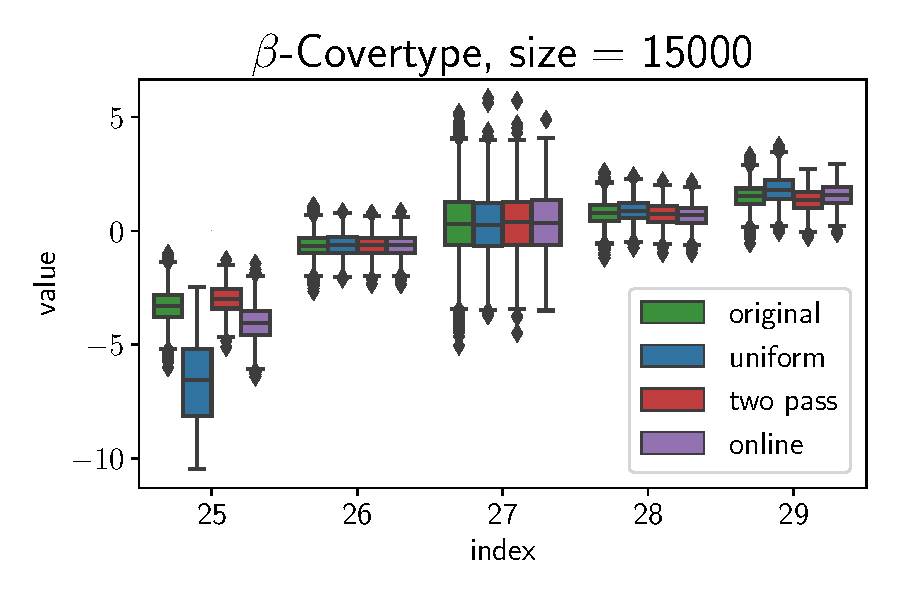
\includegraphics[width=.49\linewidth]{figures/covertype_coefficients/covertype_coefficients_25.pdf}
    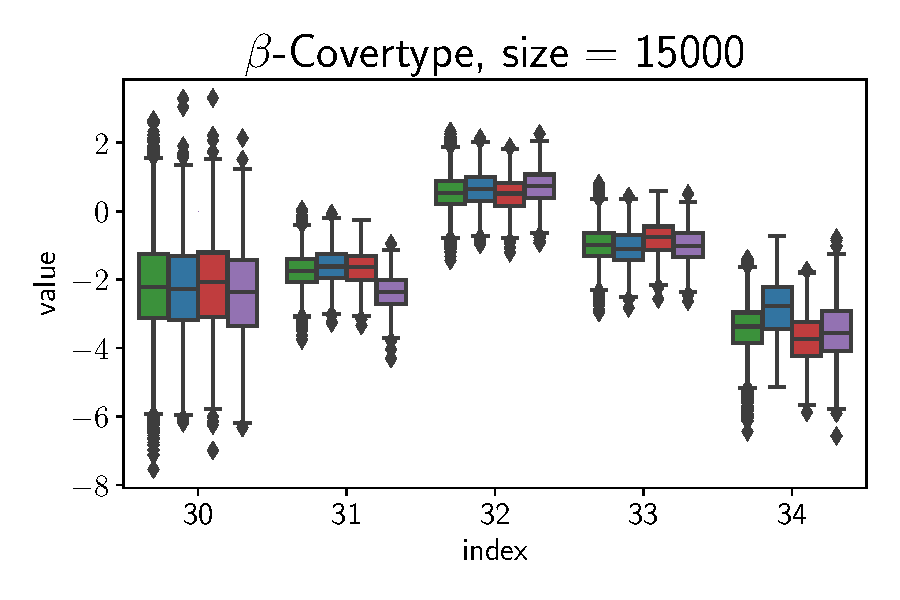
\includegraphics[width=.49\linewidth]{figures/covertype_coefficients/covertype_coefficients_30.pdf}
    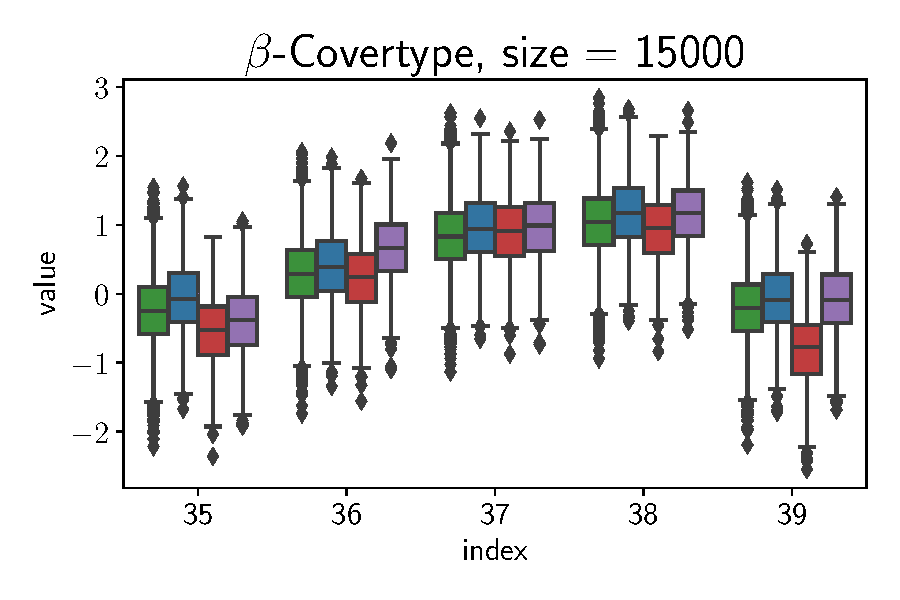
\includegraphics[width=.49\linewidth]{figures/covertype_coefficients/covertype_coefficients_35.pdf}
    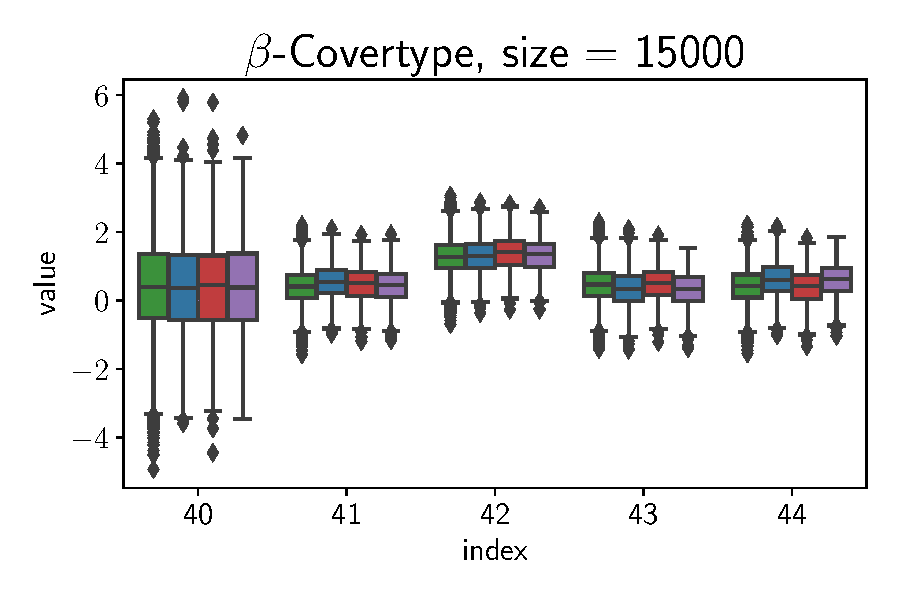
\includegraphics[width=.49\linewidth]{figures/covertype_coefficients/covertype_coefficients_40.pdf}
    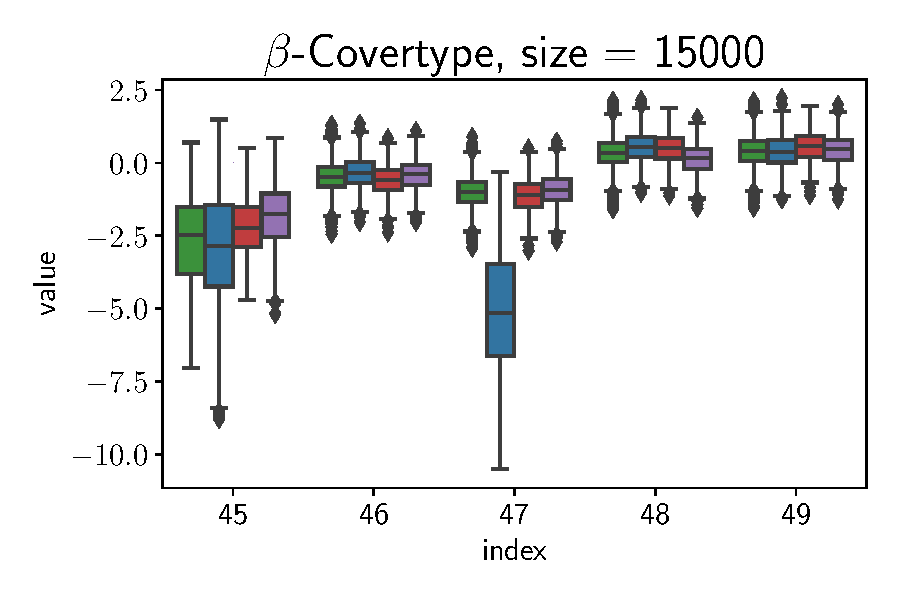
\includegraphics[width=.49\linewidth]{figures/covertype_coefficients/covertype_coefficients_45.pdf}
    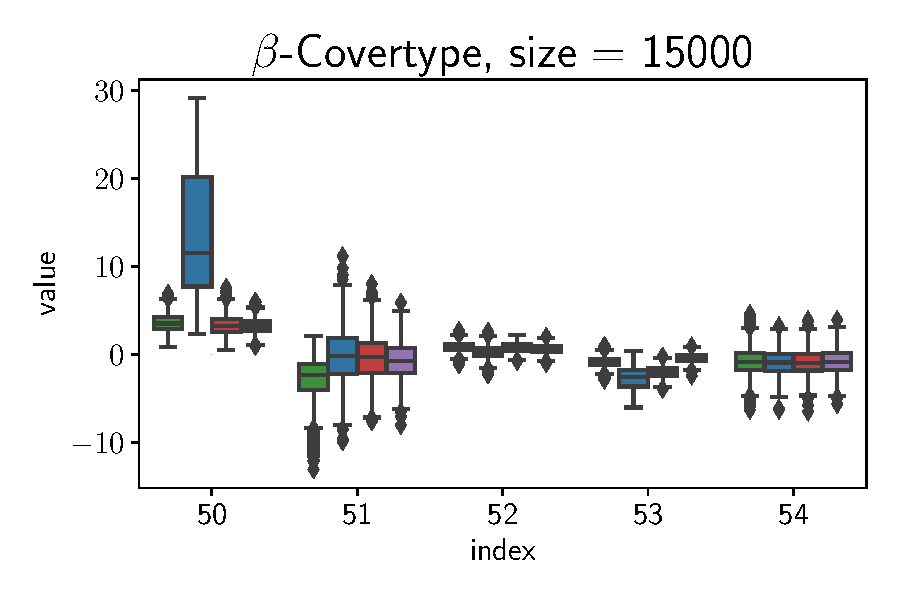
\includegraphics[width=.49\linewidth]{figures/covertype_coefficients/covertype_coefficients_50.pdf}
    \caption{The boxplots comparing the remainder $\beta_{25}$
        to $\beta_{54}$ of the posterior distributions.
        The intercept term is denoted by $\beta_{54}$.}
    \label{fig:covertype-coefficients-2}
\end{figure}

For the first coefficients, $\beta_0$ to $\beta_{8}$, we
can see that the posterior samples generated by
each of the algorithms struggle to approximate the median
as well as the variance of the original posterior distribution.
However, for the remainder of the coefficients, the approximation
seems to be very close for our two algorithms as well as for
the uniform sampling procedure, with the exception of
$\beta_{21}$, $\beta_{25}$, $\beta_{47}$ and $\beta_{50}$,
where the uniform sampling procedure fails.
Thus, we can see that for the majority of the coefficients, excluding
the coefficient $\beta_0$ to $\beta_{8}$, our algorithms already
seem to be delivering decent approximations that could potentially
even be used insead of a full posterior sample.

It remains to be investigated though, why all the algorithms struggle
with the first coefficients $\beta_0$ to $\beta_8$.
This could perhaps be due to an insufficient reduction size on
the one hand or maybe even an insufficiently small burn in value
on the other hand, but we leave this investigation as an open
problem. The most important finding of this section is, that both
of our algorithms outperform the baseline uniform sampling method
by a substantial margin.
To conclude our discussion of the experiments, we again compare
the runtimes of our algorithms, but this time for the
Bayesian setting.

\subsubsection{Comparison of Running Times}

To compare the running times of our algorithms, we take a
look at the different sampling rates, i.e.
the samples per second that the Gibbs sampler
was able to generate with and without applying our
algorithms first. The corresponding data can be found in
Table~\ref{tab:running-times-bayes}, we list the
sampling rates both including and excluding the
time it takes for the algorithms to reduce the data
before running the Gibbs sampler. We note, that for the
same reasons as in Section~\ref{sec:running-times-comparison-ml},
the online algorithm had to be excluded from the comparison.

\begin{table*}[t!]
    \centering
    \begin{tabular}{ l | l| l| l| l}
        \hline
        \textbf{Method} & \textbf{Size} & \textbf{Dataset} & \makecell{\textbf{samples / second}       \\ \textbf{(incl. red. time)}} & \makecell{\textbf{samples / second} \\ \textbf{(excl. red. time)}}\\ \hline
        No reduction    & 581012        & Covertype        & 1.5                                 & 1.5 \\ \hline
        two pass        & 15000         & Covertype        & 36                                  & 38  \\ \hline
        uniform         & 15000         & Covertype        & 46                                  & 46  \\ \hline
        two pass        & 1000          & Covertype        & 116                                 & 153 \\ \hline
        uniform         & 1000          & Covertype        & 176                                 & 176 \\ \hline
        No reduction    & 494021        & KDDCup           & 4                                   & 4   \\ \hline
        two pass        & 15000         & KDDCup           & 21                                  & 21  \\ \hline
        uniform         & 15000         & KDDCup           & 107                                 & 107 \\ \hline
        two pass        & 1000          & KDDCup           & 85                                  & 90  \\ \hline
        uniform         & 1000          & KDDCup           & 619                                 & 619 \\ \hline
        No reduction    & 350000        & Webspam          & 2                                   & 2   \\ \hline
        two pass        & 15000         & Webspam          & 13                                  & 14  \\ \hline
        uniform         & 15000         & Webspam          & 28                                  & 28  \\ \hline
        two pass        & 1000          & Webspam          & 60                                  & 62  \\ \hline
        uniform         & 1000          & Webspam          & 84                                  & 84  \\ \hline
    \end{tabular}
    \caption{The sampling rates of the Gibb sampler for
        generating the posterior samples with and without applying a data
        reduction method first.
        The sampling rates are given including and excluding the
        reduction time, i.e. the time it takes for the algorithms
        to reduce the size of the original dataset.
        We note, that for the same reasons as in
        Section~\ref{sec:running-times-comparison-ml}, the
        online algorithm was excluded from the comparison.}
    \label{tab:running-times-bayes}
\end{table*}

When looking at the sampling rates for the Covertype dataset, we can
see that both, the uniform sampling algorithm as well as our
two pass algorithm, achieve considerable speed ups for the Gibbs
sampler. While the Gibbs sampler can only generate roughly
1.5 samples every second for the full dataset, a prior reduction
to 15000 samples leads to 46 samples per second for the uniform
sampling algorithm and 36 samples per second for the two pass
algorithm (including the reduction time),
which is an increase by a factor of 30 and 24, respectively.
For reduction sizes of only 1000, we can achieve even higher
boosts of the sampling rate, but we note that the approximation
quality might not be ideal for such low reduction sizes, as
discussed in the previous section.
We can also see, that for higher reduction sizes of 15000, the
sampling rates including the reduction time are close to the
sampling rates excluding the reduction time for the two pass
algorithm, which indicates that the time it takes to reduce the
data amortizes itself the longer the Gibbs sampler runs.

It is also interesting to note, that the Gibbs sampler can generate
samples slightly quicker, when presented with a subset of the
original data that was obtained
by uniform sampling, compared to a subset of the same size
that was obtained by
the two pass algorithm.
A reason for this could perhaps be, that the leverage score based
two pass algorithm tends to pick up on outliers more frequently,
which could potentially slow down the sampling processes from
the truncated normal distribution.
In our implementation of the Gibbs sampler, the truncated normal
samples are drawn via rejection sampling, if the probability of
not rejecting a sample is sufficiently large ($\geq 5\%$), and otherwise
it falls back to a slower implementation which works better for
outliers. It could be possible, that when more outliers are present
in the reduced sample, the slower implementation is triggered more
frequently, which reduces the sampling rate.

Taking a look at the sampling rates for the Kddcup dataset,
we can observe a similar pattern,
but this time the differences between the two pass algorithm
and the uniform sampling algorithm are greater. While the
two pass algorithm for a reduction size of 15000
only achieves speed ups of a factor of
roughly 5 (including the reduction time), the uniform sampling
method allows the Gibbs sampler to increase the samples
per second by a factor of more than 26.
Here, we can see that the increased approximation quality of
the two pass algorithm doesn't come without a price. Still,
what good is the fast generation of posterior samples, if the
quality is lacking? As we saw in the previous section, the
two pass algorithm outperformed the uniform sampling method
on the Kddcup dataset in each of our quality measures.

When comparing the sampling rates of uniform sampling to the
two pass algorithm excluding the time it takes to reduce the data,
we can see even greater differences for the Kddcup dataset,
compared to Covertype.
Here it seems, that the subsets obtained by the two pass algorithm
are causing the Gibbs sampler to slow down way more than the
subsets obtained by uniform sampling.
This could potentially be explained by the fact that the Kddcup
contains a lot more outliers that the leverage score based two
pass algorithm can pick up on, which could slow down the
sampling from the truncated normal distribution.

Taking a look at the Webspam dataset, we can
see the same overall pattern that we already observed for the
other two datasets. Both, the uniform sampling procedure as well as
the two pass algorithm are able to increase the sampling rate
of the Gibbs sampler for reduction sizes of 15000 by a factor
of 6 for the two pass algorithm and 14 for uniform sampling,
including the reduction time.
However, when excluding the reduction times from the sampling
rates, the differences between uniform sampling and the two
pass algorithm aren't quite as substantial as for the Kddcup dataset,
but still higher as for the Covertype dataset.
This could, again, be due to the fact that the Webspam dataset
contains a few heavy hitters that could potentially slow down
the Gibbs sampler. On the other hand, the Webspam dataset was
shown not to be as irregular as the Kddcup dataset, which would
explain why the differences aren't that extreme.

To sum up the discussion of our experiments on coreset-based Bayesian
inference, we successfully showed that both of our algorithms
enable us to achieve a far greater approximation quality of
the posterior distribution than the uniform sampling procedure.
This increased quality comes at a price of course, because
both of our leverage score based algorithms are slower than
the uniform sampling counterpart.
It follows, that we are presented with a tradeoff:
If we choose the uniform sampling algorithm for data reduction,
we most likely get the highest increases in sampling rate for
the Gibbs sampler, but the downside is that we suffer from
instability issues and poor approximation quality.
On the other hand, if we choose one of our coreset algorithms,
we enjoy the provable guarantees of the sensitivity framework,
which lead us to more reliable and stable approximations than the
uniform sampling procedure, especially for not so well behaved
datasets like Kddcup, while still gaining decent speed ups for
the Gibbs sampler, albeit not as impressive as for the
uniform sampling.
Still, if the practitioner of a Bayesian probit analysis is faced with
the decision which data reduction algorithm to choose, he or she
will pick one of the leverage score based algorithms, if the
challenge is to obtain stable approximations of guaranteeably
high quality, while still enjoying some decent performance gains.
